%%%%%%%%%%%%%%%%%%%%%%%%%%%%%%%%%%%%%%%%%%%%%%%%%%%%%%%%%%%%
%%  This Beamer template was created by Cameron Bracken.
%%  Anyone can freely use or modify it for any purpose
%%  without attribution.
%%
%%  Last Modified: January 9, 2009
%%

\documentclass[xcolor=x11names,compress]{beamer}

%% General document %%%%%%%%%%%%%%%%%%%%%%%%%%%%%%%%%%
\usepackage{graphicx}
\usepackage{tikz}
\usetikzlibrary{decorations.fractals}
%%%%%%%%%%%%%%%%%%%%%%%%%%%%%%%%%%%%%%%%%%%%%%%%%%%%%%


%% Beamer Layout %%%%%%%%%%%%%%%%%%%%%%%%%%%%%%%%%%
\useoutertheme[subsection=false,shadow]{miniframes}
\useinnertheme{default}
\usefonttheme{serif}
\usepackage{palatino}

\setbeamerfont{title like}{shape=\scshape}
\setbeamerfont{frametitle}{shape=\scshape}

\setbeamercolor*{lower separation line head}{bg=DeepSkyBlue4} 
\setbeamercolor*{normal text}{fg=black,bg=white} 
\setbeamercolor*{alerted text}{fg=red} 
\setbeamercolor*{example text}{fg=black} 
\setbeamercolor*{structure}{fg=black} 
 
\setbeamercolor*{palette tertiary}{fg=black,bg=black!10} 
\setbeamercolor*{palette quaternary}{fg=black,bg=black!10} 

\renewcommand{\(}{\begin{columns}}
\renewcommand{\)}{\end{columns}}
\newcommand{\<}[1]{\begin{column}{#1}}
\renewcommand{\>}{\end{column}}
%%%%%%%%%%%%%%%%%%%%%%%%%%%%%%%%%%%%%%%%%%%%%%%%%%

\setbeamertemplate{footline}{%
\begin{beamercolorbox}{section in head/foot}
    \color{gray}\vskip2pt~ Johns Hopkins University\hfill\insertpagenumber{} %
    of \insertpresentationendpage{} ~\vskip2pt
\end{beamercolorbox}
}


\begin{document}


%%%%%%%%%%%%%%%%%%%%%%%%%%%%%%%%%%%%%%%%%%%%%%%%%%%%%%
%%%%%%%%%%%%%%%%%%%%%%%%%%%%%%%%%%%%%%%%%%%%%%%%%%%%%%
\section{\scshape Introduction}
\begin{frame}
\title[Copy Number]{Classification of metagenomic data}
%\subtitle{SUBTITLE}
\author{
	Shuya Chu, Stephen Cristiano, Bing He, Zhou Ye \\
	{\it Johns Hopkins University}\\
}
\date{
	\begin{tikzpicture}[decoration=Koch curve type 2] 
		\draw[DeepSkyBlue4] decorate{ decorate{ decorate{ (0,0) -- (3,0) }}}; 
	\end{tikzpicture}  
	\\
	\vspace{1cm}
	\today
}
\titlepage
\end{frame}


%%%%%%%%%%%%%%%%%%%%%%%%%%%%%%%%%%%%%%%%%%%%%%%%%%%%%%
%%%%%%%%%%%%%%%%%%%%%%%%%%%%%%%%%%%%%%%%%%%%%%%%%%%%%%
\section{\scshape Background}
%%%%%%%%%%%%%%%%%%%%%%%%%%%%%%%%%%%%%%%%%%%%%%%%%%%%%%
%%%%%%%%%%%%%%%%%%%%%%%%%%%%%%%%%%%%%%%%%%%%%%%%%%%%%%
\subsection{Biological Background}
\begin{frame}{Metagenomics}
``The application of modern genomics techniques to the study of communities of microbial organisms directly in their natural environments, bypassing the need for isolation and lab cultivation of individual species". - Lior Patcher and Kevin Chen, 2005
\end{frame}
%%%%%%%%%%%%%%%%%%%%%%%%%%%%%%%%%%%%%%%%%%%%%%%%%%%%%%
%%%%%%%%%%%%%%%%%%%%%%%%%%%%%%%%%%%%%%%%%%%%%%%%%%%%%%
\begin{frame}{Biological motivation}

\begin{itemize}
	\item Potential impact on public health (the human microbiome project), agriculture, biofuels, and other fields.
	\item If we take an environmental sample (soil, gut, $\ldots$) and sequence the contained DNA, we will generate reads from many microbial organisms. 
	\item We wish to classify each read to its correct phylogenic origin and gain some insight to the abundance of each organism within the sample.
	\item Complicated by the hierarchical structure of the classifications and since in a metagenomic sample, many reads will come from \emph{``de novo"} genomes.
\end{itemize}
\end{frame}
%%%%%%%%%%%%%%%%%%%%%%%%%%%%%%%%%%%%%%%%%%%%%%%%%%%%%%
%%%%%%%%%%%%%%%%%%%%%%%%%%%%%%%%%%%%%%%%%%%%%%%%%%%%%%
\subsection{Existing Methods}
\begin{frame}{Existing Methods}
\begin{itemize}
	\item PhymmBL
		\begin{itemize}
			\item Arthur Brady and Steven Salzberg 
			\item Uses Interpolated Markov Model together with BLAST to classify DNA taxonomically classify metagenomic reads.
			\item Very accurate, but local alignment with BLAST is very slow!
		\end{itemize}
	\item FACS
	\begin{itemize}
			\item Henrik Stranneheim and Joakim  Lundeberg
			\item Bloom Filter approach - very space-efficient.
			\item Has performance issues and primary purpose is identifying DNA contamination in metagenome sample.
		\end{itemize}
	\item Kraken
		\begin{itemize}
			\item Derick Wood and Steven Salzberg
			\item Novel classification algorithm utilizing exact alignment of k-mers.
			\item Achieves very high speed in exchange for a slight sacrifice of sensitivity.
		\end{itemize}
		\item MetaPhlAn, MEGAN, metaphyler, $\ldots$
	\end{itemize}
\end{frame}
%%%%%%%%%%%%%%%%%%%%%%%%%%%%%%%%%%%%%%%%%%%%%%%%%%%%%%
%%%%%%%%%%%%%%%%%%%%%%%%%%%%%%%%%%%%%%%%%%%%%%%%%%%%%%
\subsection{Data}
\begin{frame}{Data}
\begin{columns}[c] % The "c" option specifies centered vertical alignment while the "t" option is used for top vertical alignment

\column{.45\textwidth} % Left column and width
\begin{itemize}\itemsep1em
\item RefSeq for whole genomes of bacteria (obtained from NCBI)
\item Due to vastness of RefSeq, only considered proteobacterium phylum.
\item Generated simulated FASTA files from Metasim and some of our own scripts.
\end{itemize}

\column{.5\textwidth} % Right column and width
         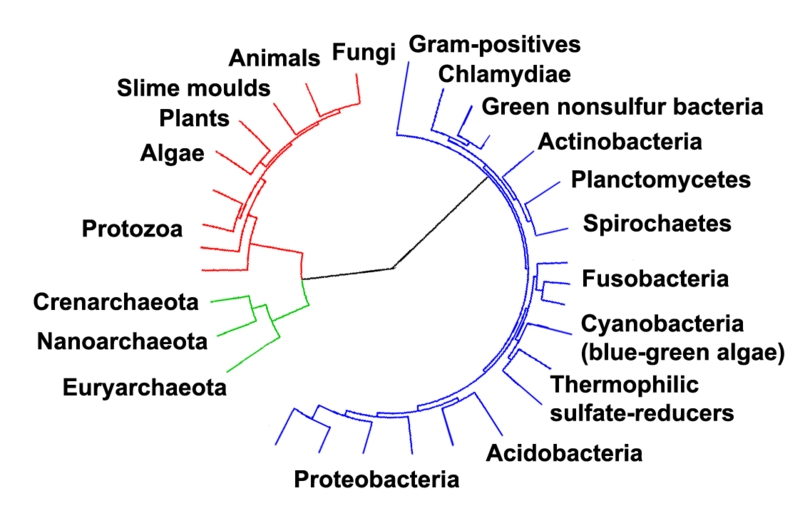
\includegraphics[width=1\textwidth, height=1\textwidth]{phylogeny.png}\\
\end{columns}

\end{frame}
%%%%%%%%%%%%%%%%%%%%%%%%%%%%%%%%%%%%%%%%%%%%%%%%%%%%%%
%%%%%%%%%%%%%%%%%%%%%%%%%%%%%%%%%%%%%%%%%%%%%%%%%%%%%%
\section{\scshape Bloom Filter}
\subsection{}
%%%%%%%%%%%%%%%%%%%%%%%%%%%%%%%%%%%%%%%%%%%%%%%%%%%%%%
%%%%%%%%%%%%%%%%%%%%%%%%%%%%%%%%%%%%%%%%%%%%%%%%%%%%%%
\begin{frame}{Bloom Filter}
\begin{center}
         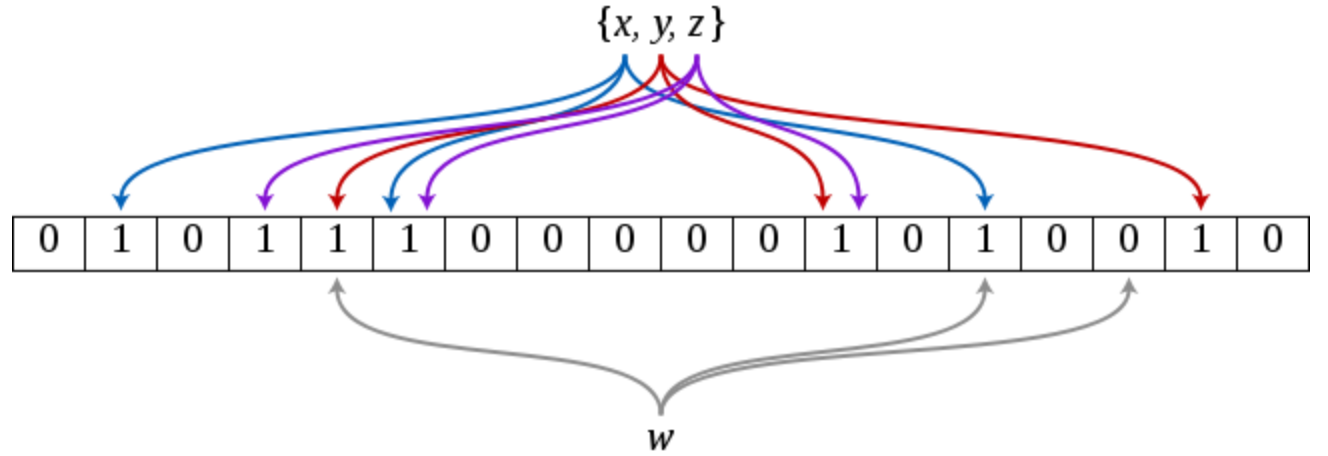
\includegraphics[width=0.8\textwidth, height=0.3\textwidth]{Bloom_filter.png}\\
\end{center}
Recall: a Bloom filter is a sketch data structure that is extremely compact, but fails sometimes.
\par
We use the PERL module Bloom::Faster to build bloom filters from our reference genomes.
\begin{center}
         
\includegraphics[width=1\textwidth, height=0.05\textwidth]{bloomfaster.png}\\
\end{center}
\end{frame}

%%%%%%%%%%%%%%%%%%%%%%%%%%%%%%%%%%%%%%%%%%%%%%%%%%%%%%
%%%%%%%%%%%%%%%%%%%%%%%%%%%%%%%%%%%%%%%%%%%%%%%%%%%%%%
\begin{frame}{Bloom Filter}
General Process
\begin{itemize}
\item {\bf First}, split query seq into K-mers (with the same length we used to build the filter). {\bf Second}, query K-mers against each Bloom Filter for each Ref Genome.
\item {\bf Coarse Scan}: Query Bloom Filter with Non-overlapping K-mers. 
\item {\bf Detailed Scan}: If query seq passes the Coarse Scan, we query Bloom Filter all (overlapping) K-mers.
\end{itemize}
Scoring
\begin{itemize}
	\item Match score proportional to matched bp in each query seq.
	\item {\bf Species level}: combine max and threshold for match score.
	\item {\bf Higher level}: if species-level classification cannot be made, use mutual information criteria for classifying at genus (or higher) level.
	\item Incorporate false positive rate into match score?
\end{itemize}


\end{frame}
%%%%%%%%%%%%%%%%%%%%%%%%%%%%%%%%%%%%%%%%%%%%%%%%%%%%%%
%%%%%%%%%%%%%%%%%%%%%%%%%%%%%%%%%%%%%%%%%%%%%%%%%%%%%%
\begin{frame}{Preliminary Results}
\begin{columns}[c] % The "c" option specifies centered vertical alignment while the "t" option is used for top vertical alignment

\column{.45\textwidth} % Left column and width
Query simulated data with Exact model: \\
Takes 43 seconds \\
\vspace{0.5cm}
		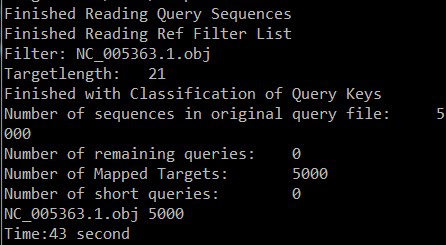
\includegraphics[width=1\textwidth, height=0.84\textwidth]{bloomresults1.png}\\
\column{.5\textwidth} % Right column and width
Query simulated data with 454 error model: \\
Takes 8 seconds \\
\vspace{0.5cm}
         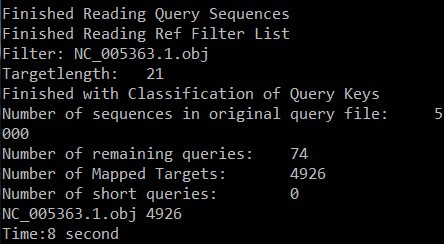
\includegraphics[width=1\textwidth, height=0.75\textwidth]{bloomresults2.png}\\
\end{columns}

\end{frame}
%%%%%%%%%%%%%%%%%%%%%%%%%%%%%%%%%%%%%%%%%%%%%%%%%%%%%%
%%%%%%%%%%%%%%%%%%%%%%%%%%%%%%%%%%%%%%%%%%%%%%%%%%%%%%
\section{\scshape Markov Model}
\subsection{}
\begin{frame}{Interpolated Markov Model}
For modeling DNA, we need $O(4^{n+1})$ parameters for an n-th order Markov model.

Interpolated Markov model combines the merits of both low and high order Markov model. 

Basic Model:
\begin{equation*}
\begin{aligned}
&P_{IMM}(x_i | x_{i-1}, \cdots, x_{i-n})\\
&= \lambda_0P(x_i)+\lambda_1P(x_i | x_{i-1})+\cdots+\lambda_nP(x_i | x_{i-1}, \cdots, x_{i-n})
\end{aligned}
\end{equation*}
where $\sum_{i}\lambda_i = 1$

Improved Model (Use History):
\begin{equation*}
\begin{aligned}
&P_{IMM, n}(x_i | x_{i-1}, \cdots, x_{i-n})\\
&= \lambda_n(x_i)P(x_i | x_{i-1}, \cdots, x_{i-n})\\
&+(1-\lambda_n(x_i))P_{IMM, n-1}(x_i | x_{i-1}, \cdots, x_{i-n+1})
\end{aligned}
\end{equation*}
\end{frame}

\begin{frame}
\frametitle{Parameter Learning}
We learn the probability $P(x_i | x_{i-1}, \cdots, x_{i-n})$ by counting. 

\begin{equation*}
P(x_i | x_{i-1}, \cdots, x_{i-n}) = \frac{f(x_i, x_{i-1}, \cdots, x_{i-n})}{f(x_{i-1}, \cdots, x_{i-n})}
\end{equation*}
where $f$ is the number of occurrences of input string

$\lambda$ is determined by a $\chi^2$ hypothesis test. If there are sufficient number of strings $c$ to compute $P(x_i | x_{i-1}, \cdots, x_{i-n})$, we set $\lambda_n(x_i)$ as $1$; otherwise, we compare the distribution of n-th order history and n-1-th by $\chi^2$ hypothesis test. After doing this test, we will obtain a p-value $d$. We determine $\lambda_n(x_i)$ by:

\begin{equation*}
\lambda_n(x_i) = 
\begin{cases}
1.0	& \text{if } c > threshold \\
\frac{c}{400} \times d & \text{if } d \ge 0.05, c \le threshold\\
0.0 & \text{if } d < 0.05, c \le threshold
\end{cases}
\end{equation*}

The threshold is determined by trial and error. 
\end{frame}


%%%%%%%%%%%%%%%%%%%%%%%%%%%%%%%%%%%%%%%%%%%%%%%%%%%%%%
%%%%%%%%%%%%%%%%%%%%%%%%%%%%%%%%%%%%%%%%%%%%%%%%%%%%%%
\section{\scshape Bowtie}
\subsection{}
\begin{frame}{Improvement with Bowtie}
What is Bowtie?
\begin{itemize}
	\item Bowtie is a sequence aligner wrote by professor Langmead. 
	\item  It indexes the genome with an FM Index to align short reads.
	\item  For each alignment, Bowtie also scores them
\end{itemize}

Idea for Improvement:
\begin{itemize}
	\item Using score for previous alignment, skip some bad alignment
	
	\item Details: If the sample data get a `bad' score when aligning to a species, then it definitely will have bad scores for the species in the same genus. 
	\end{itemize}
\end{frame}
%%%%%%%%%%%%%%%%%%%%%%%%%%%%%%%%%%%%%%%%%%%%%%%%%%%%%%
%%%%%%%%%%%%%%%%%%%%%%%%%%%%%%%%%%%%%%%%%%%%%%%%%%%%%%
\begin{frame}{Improvement with Bowtie}
Set the Threshold:
\begin{itemize}
     \item Give more penalties for mismatch(gap)
	\item  Use the average score 
\end{itemize}

Ongoing work:
\begin{itemize}
	\item Still thinking about how to get the best threshold
	\item Comparison and analysis between this and bowtie 
\end{itemize}
\end{frame}

%%%%%%%%%%%%%%%%%%%%%%%%%%%%%%%%%%%%%%%%%%%%%%%%%%%%%%
%%%%%%%%%%%%%%%%%%%%%%%%%%%%%%%%%%%%%%%%%%%%%%%%%%%%%%
\section{\scshape Ongoing work}
\subsection{}
\begin{frame}{Ongoing work}
\begin{itemize}
	\item Benchmark all the methods against each other on the same machine and input.
	\item Memory footprint of bloom filter vs Markov Model.
	\item Instead of absolute classification, return a confidence score instead.
	\item Investigate how well a method deals with \emph{de novo} genomes.
\end{itemize}

\end{frame}
%%%%%%%%%%%%%%%%%%%%%%%%%%%%%%%%%%%%%%%%%%%%%%%%%%%%%
%%%%%%%%%%%%%%%%%%%%%%%%%%%%%%%%%%%%%%%%%%%%%%%%%%%%%%
\begin{frame}{Thanks}
\begin{itemize}\itemsep1em
	\item Ben Langmead
	\item The developers of the open source software which aided us in this project.
	\item Hongkai Ji and Kasper Hansen
\end{itemize}

\end{frame}
\end{document}